% We're writing an "article." Set margins.
\documentclass[11pt]{article}
\usepackage[margin=1in]{geometry}

% Adjust fonts, re-set the proof tombstone symbol, adjust paragraph indents
% and skips.
\usepackage{amsmath,amssymb,amsthm,nicefrac,mathtools}
\usepackage{xspace,multicol}
\usepackage{amsfonts,mathrsfs,amsbsy,textcomp,twemojis}		% Fancy script stuff.

\usepackage{aurical}						% Auriocus Kalligraphicus.
%\usepackage{tgpagella}						% TeX Gyre Pagella
%\usepackage{tgschola}						% TeX Gyre Schola
\usepackage{baskervillef}					% BaskervilleF
%\usepackage{baskervald}					% Baskervald ADF
%\usepackage[lf]{Baskervaldx}				% Baskervald X
%\usepackage{librebaskerville}				% Libre Baskerville (too big?)
%\renewcommand*\familydefault{\sfdefault}	% CMU Sans-Serif, roman math
%\usepackage{libertine}						% Linux Libertine

%\renewcommand{\qedsymbol}{
%	\raisebox{-\baselineskip}{\llap{\twemoji[scale=0.5]{swan}}}
%}	% Swan tombstone.

%\renewcommand{\qedsymbol}{
%	\raisebox{-\baselineskip}{\textleaf}
%}	% Leaf; doesn't seem to work with baskervald? not sure why.

\renewcommand{\qedsymbol}{
	\raisebox{-\baselineskip}{\llap{\twemoji[scale=0.5]{stop sign}}}
}	% Stop sign.

\setlength{\parindent}{0em}		% No paragraph indents.
\setlength{\parskip}{1em}		% Single-line paragraph skips.


% Math symbols, nice fractions, theorem environments.
\theoremstyle{definition}
\newtheorem*{theorem*}{Theorem}
\newtheorem*{definition*}{Definition}
\newtheorem{definition}{Definition}
\newtheorem*{definitions*}{Definitions}
\newtheorem*{conjecture*}{Conjecture}

\newcommand{\R}{\mathbb{R}}			% Reals.
\newcommand{\N}{\mathbb{N}}			% Naturals.
\newcommand{\Z}{\mathbb{Z}}			% Integers.
\newcommand{\Q}{\mathbb{Q}}			% Rationals.
\renewcommand{\H}{\mathbb{H}}		% Hamiltonian quaternions.
\newcommand{\C}{\mathbb{C}}			% Complex.
\renewcommand{\P}{\mathbb{P}}		% Polynomials.
\newcommand{\F}{\mathbb{F}}			% General field.

\newcommand{\Aut}[2][]{\mathbf{Aut}_{#1}\hspace{-2pt}\left(#2\right)}	% Automorphism group with an optional categorical argument.
\newcommand{\Sym}[1]{\mathbf{Sym}\hspace{-2pt}\left(#1\right)}			% Symmetric group.
\newcommand{\Hom}[2][]{\mathbf{Hom}_{#1}\hspace{-2pt}\left(#2\right)}	% Hom-set with an optional categorical argument.
\newcommand{\GL}[2][n]{\mathbf{GL}_{#1}\hspace{-2pt}\left(#2\right)}	% General linear group with an optional dimensional argument.
\newcommand{\Kernel}[1]{\mathrm{Ker}\ #1}		% Kernel.
\newcommand{\Image}[1]{\mathrm{Im}\ #1}			% Image.
\newcommand{\Rank}[1]{\operatorname{Rank} #1}	% Rank.
\newcommand{\Set}{\textbf{Set}}					% "Set" category.
\newcommand{\Vect}{\textbf{Vect}}				% "Vector space" category.
\newcommand{\Grp}{\textbf{Grp}}					% "Group" category.
\newcommand{\Ab}{\textbf{Ab}}					% "Abelian group" category.
\newcommand{\id}{\textbf{id}}					% Alternate identity map notation.

\newcommand{\coo}{c_{00}}			% Sequence space: vectors have finitely many nonzero entries.
\newcommand{\co}{c_0}				% Sequence space: vector entries converge to zero.
\newcommand{\Poly}{P([0,1])}		% Polynomials over [0,1].
\newcommand{\Cont}{C^1([0,1])}		% Once-differentiable functions over [0,1].

\newcommand{\norm}[2][\infty]{\left\lVert #2 \right\rVert_{#1}} 	% Norm; optional p-norm argument.

\newcommand{\inverse}[1]{#1^{-1}}			% Inverse.
\let\preimage=\inverse						% Preimage.
\newcommand{\pp}[1]{#1^{\prime}}			% Prime.
\newcommand{\conjugate}[1]{\overline{#1}}	% Conjugate.
\let\complement=\conjugate					% Complement.
\newcommand{\closure}[1]{
	\text{cl}\hspace{-2pt}\left(#1\right)	% Closure.
}
\newcommand{\interior}[1]{\operatorname{int}\left(#1\right)}	% Interior.
\newcommand{\boundary}[1]{\operatorname{bd}\left(#1\right)}		% Boundary.

\newcommand{\pset}[1]{\raisebox{.15\baselineskip}{\Large\ensuremath{\wp}\hspace{-1.5pt}}\left(#1\right)}	% Insane power set symbol.

\newcommand{\Mod}[1]{\hspace{0.2em}(\mathrm{mod}\ #1)}	% Properly formatted modulus.
\newcommand{\divides}{\hspace{0.2em} | \hspace{0.2em}}	% Scalable divides.

\newcommand{\topology}{\text{\Fontauri\bfseries T}\hspace{1pt}}	% Fancy topology symbol.

\newcommand{\probability}[1]{\operatorname{\mathbf P}\left[#1\right]}	% Probability symbol.
\newcommand{\betti}{\mathbf{b}}									% Betti number symbol.
\newcommand{\expectation}[1]{\mathbb{E}\left[#1\right]}			% Expectation.
\newcommand{\area}[1]{\operatorname{Area}\left(#1\right)}		% Area, perimeter.
\newcommand{\perimeter}[1]{\operatorname{Perim}\left(#1\right)}


% Tools for colors, pictures, diagrams, lists, and adjusting widths.
\usepackage{tikz,xcolor,enumitem,quiver,adjustbox,placeins,float}
\usetikzlibrary{graphs,graphs.standard,calc}
\newcommand{\tast}{\textasteriskcentered}			% New asterisk symbol.


% Proof and theorem framing.
\usepackage[framemethod=tikz]{mdframed}

\mdfsetup{skipbelow=0pt}			% Skip no additional space below the frame.

\mdfdefinestyle{proof}{
	innertopmargin=1em,			% Single-line spacing from the top of the frame.
	innerbottommargin=1em,		% Single-line spacing to the frame bottom.
	linecolor=black,			% Black lines, 1pt in width.
	linewidth=1pt,
	align=center,				% Align the frame in the center of the page.
	leftmargin=0.05\textwidth,	% Margin from the left.
	skipabove=1.5em				% 1.5 lines of space from content to frame.
}
\surroundwithmdframed[style=proof]{definition}
\surroundwithmdframed[style=proof]{definitions}
\surroundwithmdframed[style=proof]{definitions*}
\surroundwithmdframed[style=proof]{definition*}

\mdfdefinestyle{theorem}{
	innertopmargin=1em,			% Single-line spacing from the top of the frame.
	innerbottommargin=1em,		% Single-line spacing to the frame bottom.
	linecolor=bured,			% Black lines, 1pt in width.
	linewidth=2pt,
	align=center,				% Align the frame in the center of the page.
	leftmargin=0.05\textwidth,	% Margin from the left.
	skipabove=1.5em				% 1.5 lines of space from content to frame.
}

\surroundwithmdframed[style=theorem]{proof}		% Proofs, theorems, definitions.
\surroundwithmdframed[style=theorem]{theorem*}
\surroundwithmdframed[style=theorem]{conjecture*}


% Note-taking. %
\definecolor{brightlavender}{rgb}{0.75, 0.58, 0.89}
\definecolor{bured}{rgb}{0.8, 0.0, 0.0}
\definecolor{amber}{rgb}{1.0, 0.75, 0.0}
\definecolor{amethyst}{rgb}{0.6, 0.4, 0.8}
\definecolor{azure}{rgb}{0.0, 0.5, 1.0}
\definecolor{amaranth}{rgb}{0.9, 0.17, 0.31}

\newcommand{\question}[1]{{\color{brightlavender}\textit{\textbf{(#1)}}}}
\newcommand{\thepoint}[1]{{\color{azure}\textit{\textbf{#1}}}}
\newcommand{\comment}[1]{{\color{bured}\textit{\textbf{#1}}}}

% Random numbers?
\usepackage[first=0,last=1]{lcg}

\newcommand{\newrandomvar}[1]{%
	\newcommand{#1}{}
	\rand
	\edef#1{\arabic{rand}}
}

\pgfmathdeclarerandomlist{Checkers}{%
    {bured}%
    {black}%    
}%


% Set up captions.
\usepackage{caption}
\captionsetup{
	labelformat=empty,
	width=0.9\linewidth,
	font={it,small}
}

% Nice footnotes.
\usepackage[hang,flushmargin]{footmisc}


\begin{document}

	\section*{Beginnings}
		Consider the following graph $G$:
		\begin{center}
			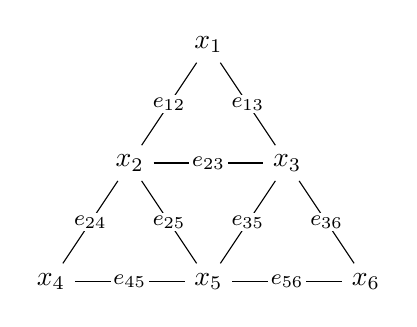
\begin{tikzpicture}
				\graph [no placement, edge quotes={fill=white, inner sep=1pt}] {
					x4/$x_4$[x=0,y=0] --["\footnotesize$e_{45}$"] x5/$x_5$[x=2,y=0] --["\footnotesize$e_{56}$"] x6/$x_6$[x=4,y=0],
					x2/$x_2$[x=1,y=1.5] --["\footnotesize$e_{23}$"] x3/$x_3$[x=3,y=1.5],
					x1/$x_1$[x=2,y=3],
					x1 --["\footnotesize$e_{12}$"] x2, x1 --["\footnotesize$e_{13}$"] x3,
					x2 --["\footnotesize$e_{24}$"] x4, x2 --["\footnotesize$e_{25}$"] x5,
					x3 --["\footnotesize$e_{35}$"] x5, x3 --["\footnotesize$e_{36}$"] x6
				};
			\end{tikzpicture}
		\end{center}	

		\begin{definitions*}[Chains, boundary, coboundary]
			Recall that $C_0$ is the free abelian group generated by the set of vertices of $G$; each of these elements is a \textit{$0$-dimensional chain} or \textit{$0$-chain}. $C_1$ is the free abelian group generated by the set of (possibly directed) edges; each of these elements is called a \textit{$1$-dimensional chain} or \textit{$1$-chain}.
			
			The \textit{boundary operator} $\partial$ sends $1$-chains to $0$-chains, and the \textit{coboundary operator} $\delta$ sends $0$-chains to $1$-chains: that is, $$ \partial : C_1 \to C_0 \text{ and } \delta : C_0 \to C_1. $$ Each is linear; for $x=uv$ an edge of $G$, $$ \partial(uv) = u + v,$$ which is a $0$-chain; for $u$ a vertex of $G$, $$ \delta(u) = \sum \varepsilon_i x_i,$$ where $\varepsilon_i$ is $1$ whenever (the edge) $x_i$ is incident to $u$. A \textit{coboundary} is the coboundary of some $0$-chain in $G$.
		\end{definitions*}
		
		A $0$-chain $\sigma$ in $G$ is $$\sigma = x_1 + x_2 + x_3$$ and has as its coboundary
		\begin{align*}
 			\delta(\sigma) &= (e_{12} + e_{13}) + (e_{12} + e_{23} + e_{24} + e_{25}) + (e_{13} + e_{23} + e_{35} + e_{36}) \\
 			&= 2e_{12} + 2e_{13} + 2e_{23} + e_{24} + e_{25} + e_{35} + e_{36} \\
 			&= e_{24} + e_{25} + e_{35} + e_{36}.
		\end{align*}
		
		Graphically, we have
		
		\begin{center}
			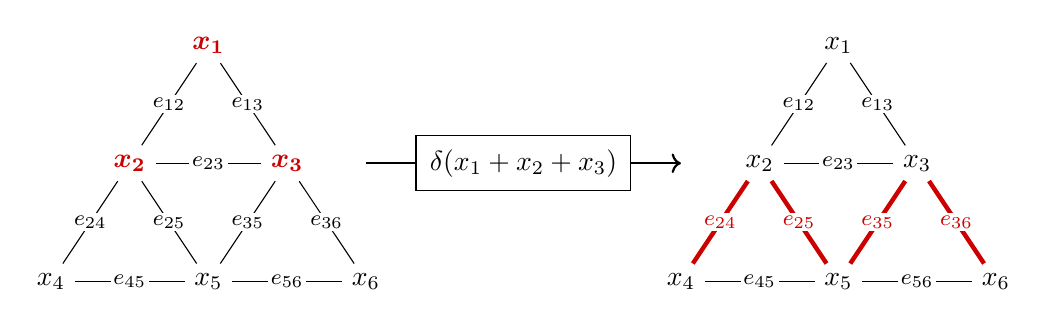
\begin{tikzpicture}
				\graph [no placement, edge quotes={fill=white, inner sep=1pt}] {
					x4/$x_4$[x=0,y=0] --["\footnotesize$e_{45}$"] x5/$x_5$[x=2,y=0] --["\footnotesize$e_{56}$"] x6/$x_6$[x=4,y=0],
					x2/$\color{bured}\boldsymbol{x_2}$[x=1,y=1.5] --["\footnotesize$e_{23}$"] x3/$\color{bured}\boldsymbol{x_3}$[x=3,y=1.5],
					x1/$\color{bured}\boldsymbol{x_1}$[x=2,y=3],
					x1 --["\footnotesize$e_{12}$"] x2, x1 --["\footnotesize$e_{13}$"] x3,
					x2 --["\footnotesize$e_{24}$"] x4, x2 --["\footnotesize$e_{25}$"] x5,
					x3 --["\footnotesize$e_{35}$"] x5, x3 --["\footnotesize$e_{36}$"] x6
				};
			
				\draw [->,thick](4, 1.5) -- (8, 1.5);
				\draw node[draw, inner sep=5pt, align=center, fill=white] at (6,1.5) {$\delta(x_1 + x_2 + x_3)$};
				
				\graph [no placement, edge quotes={fill=white, inner sep=1pt}] {
					x4/$x_4$[x=8,y=0] --["\footnotesize$e_{45}$"] x5/$x_5$[x=10,y=0] --["\footnotesize$e_{56}$"] x6/$x_6$[x=12,y=0],
					x2/$x_2$[x=9,y=1.5] --["\footnotesize$e_{23}$"] x3/$x_3$[x=11,y=1.5],
					x1/$x_1$[x=10,y=3],
					x1 --["\footnotesize$e_{12}$"] x2, x1 --["\footnotesize$e_{13}$"] x3,
					x2 --[ultra thick,"\footnotesize$e_{24}$",bured] x4, x2 --[ultra thick, bured, "\footnotesize$e_{25}$"] x5,
					x3 --[ultra thick, bured, "\footnotesize$e_{35}$"] x5, x3 --[ultra thick, bured, "\footnotesize$e_{36}$"] x6
				};
			\end{tikzpicture}	
		\end{center}
		
		For a $1$-chain like $\omega = e_{12} + e_{13}$, we have
			\begin{align*}
				\partial(\omega) &= \partial(e_{12} + e_{13}) \\
				&= \partial(e_{12}) + \partial(e_{13}) \\
				&= (x_1 + x_2) + (x_1 + x_3) \\
				&= 2x_1 + x_2 + x_3	\\
				&= x_2 + x_3.
			\end{align*}
			
		Graphically, we get
		
		\begin{center}
			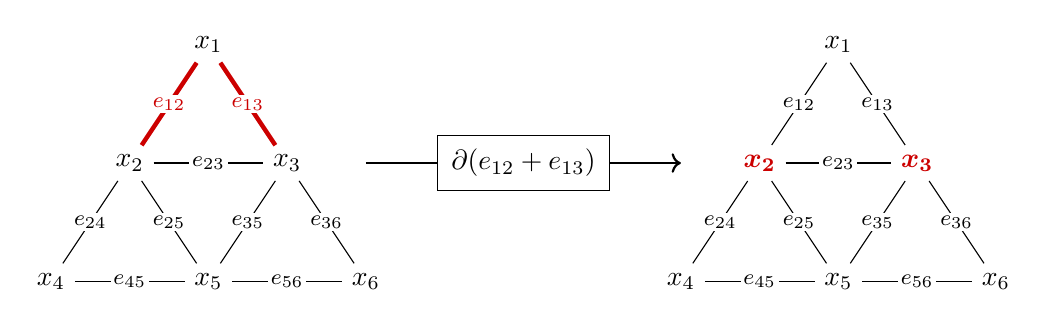
\begin{tikzpicture}
				\graph [no placement, edge quotes={fill=white, inner sep=1pt}] {
					x4/$x_4$[x=0,y=0] --["\footnotesize$e_{45}$"] x5/$x_5$[x=2,y=0] --["\footnotesize$e_{56}$"] x6/$x_6$[x=4,y=0],
					x2/$x_2$[x=1,y=1.5] --["\footnotesize$e_{23}$"] x3/$x_3$[x=3,y=1.5],
					x1/$x_1$[x=2,y=3],
					x1 --[ultra thick, bured, "\footnotesize$e_{12}$"] x2, x1 --[ultra thick, bured, "\footnotesize$e_{13}$"] x3,
					x2 --["\footnotesize$e_{24}$"] x4, x2 --["\footnotesize$e_{25}$"] x5,
					x3 --["\footnotesize$e_{35}$"] x5, x3 --["\footnotesize$e_{36}$"] x6
				};
							
				\draw [->,thick](4, 1.5) -- (8, 1.5);
				\draw node[draw, inner sep=5pt, align=center, fill=white] at (6,1.5) {$\partial(e_{12} + e_{13})$};
				
				\graph [no placement, edge quotes={fill=white, inner sep=1pt}] {
					x4/$x_4$[x=8,y=0] --["\footnotesize$e_{45}$"] x5/$x_5$[x=10,y=0] --["\footnotesize$e_{56}$"] x6/$x_6$[x=12,y=0],
					x2/$\color{bured}\boldsymbol{x_2}$[x=9,y=1.5] --["\footnotesize$e_{23}$"] x3/$\color{bured}\boldsymbol{x_3}$[x=11,y=1.5],
					x1/$x_1$[x=10,y=3],
					x1 --["\footnotesize$e_{12}$"] x2, x1 --["\footnotesize$e_{13}$"] x3,
					x2 --["\footnotesize$e_{24}$"] x4, x2 --["\footnotesize$e_{25}$"] x5,
					x3 --["\footnotesize$e_{35}$"] x5, x3 --["\footnotesize$e_{36}$"] x6
				};
			\end{tikzpicture}	
		\end{center}

		
		Basically, \thepoint{the coboundary operator sends sets of vertices $V_\sigma$ to the set of edges $E_\sigma$ incident to exactly one of the vertices in $V_\sigma$,} while \thepoint{the boundary operator sends sets of edges $E_\omega$ to the set of vertices $V_\omega$ incident to exactly one of the edges in $E_\omega$}. Note that our addition here is over $\F_2$ ($\cong \Z_2 \cong \Z/2\Z$). 
		
		\begin{definitions*}[Cycle vector, cycle space, cutset, cocycle, cocycle space]
			A $1$-chain with boundary $0$ is called a \textit{cycle vector} and is a collection of edge-disjoint cycles; each cycle vector belongs to the \textit{cycle space} of $G$, a vector space over $\F_2$. The \textit{cycle basis} for the cycle space of $G$ is the set of cycles $Z(T)$: $Z(T)$ is the set of minimal cycles induced by adjoining, one-by-one, each edge in the cotree $T^*$. These cycles are independent, as each of them differs by at least one edge. Any cycle $Z$ in the cycle space of $T$ can be written as $$ \sum_{i=1}^k \varepsilon_i C_i,$$ where $\varepsilon_i = 1$ if $Z$ shares boundary \question{or point? not sure} with $C_i$.
			
			A \textit{coboundary} of $G$ is the coboundary of some $0$-chain in $G$. A \textit{cutset} of a connected graph $G$ is a collection of edges that, when deleted, disconnects $G$. Every coboundary is a cutset, as the coboundary of any vertex $x_i$ is simply the edges to all its neighbors; when the coboundary is deleted, $x_i$ is an isolated point. A \textit{cocycle} is, equivalently: a minimal cutset of $G$; a minimal nonzero coboundary. The collection of cocycles is called the \textit{cocycle space}; given a spanning tree $T$, the set of cocycles constructed by adding a single edge \textit{not} in $T^*$ serves as a basis for this space.
		\end{definitions*}
		
		\begin{definitions*}[The above, more generally]
			We can even couch the above definitions in more topological language. Let an \textit{$n$-simplex} be the $n$-dimensional analogue of a triangle: for example, the \textit{standard $n$-simplex} is defined by $$\Delta^n = \left\{(t_0, \dots, t_n) \in \R^{n+1} : \sum t_i = 1 \hspace{1em} \text{and} \hspace{1em} t_i \geq 0\right\}. $$ The group $\Delta_n(X)$ is then the free abelian group generated by the (``open,'' i.e. with faces deleted) $n$-simplices.
			
			A \textit{$\Delta$-complex} is just a bunch of simplices glued together; more precisely, it's the quotient space of simplices we get by identifying faces. Note that vertices ($0$-simplices) are ordered by the orientations of their edges ($1$-simplices); higher-dimensional simplices can be ordered as well. An \textit{$n$-chain} is a linear combination of $n$-simplices in a complex, and the \textit{boundary homomorphism} $\partial_n : \Delta_n(X) \to \Delta_{n+1}(X)$ sends $n$-chains to $(n-1)$-chains as given by $$ \partial_n(\sigma) = \sum_{k} (-1)^k (v_0, \dots, \hat v_k, \dots, v_n), $$ where ``$\hat v_k$'' indicates that the $k$\textsuperscript{th} vertex was deleted from the sequence of vertices $v_0, \dots, v_n$. Note that the composition $\partial_n \circ \partial_{n+1}$ (often written using juxtaposition, as $\partial_n\partial_{n+1}$) is always zero by the linearity of the $\partial$ operator, as the signs of each face are swapped.
			
			Using these operators, we get a \textit{sequence of homomorphisms of abelian groups} $$ \cdots \longrightarrow C_{n+1} \overset{\partial_{n+1}}{\longrightarrow} C_n \overset{\partial_n}{\longrightarrow} C_{n-1} \longrightarrow \cdots \overset{\partial_1}{\longrightarrow} C_0 \overset{\partial_0}{\longrightarrow} 0, $$ called a \textit{chain complex} (where $C_n$ is a free abelian group on some basis of $n$-simplices; it's possible that $C_n = \Delta_n(X)$). Recalling that $\partial_n\partial_{n+1} = 0$, we know that $\partial_{n}$ sends everything in $\Image \partial_{n+1}$ to $0$, so $\Image \partial_{n+1} \subseteq \Kernel \partial_n$. The \textit{$n$\textsuperscript{th} homology group} is then $H_n = \Kernel \partial_n / \Image \partial_{n+1}$, which gives us a way to classify \textit{cycles} (elements of $\Kernel \partial_n$) by the \textit{boundaries} (elements of $\Image \partial_{n+1}$) to which they belong; elements of $H_n$ are called \textit{homology classes}, and two cycles representing the same boundary are \textit{homologous}.
			
			If we want to go in the reverse direction (i.e. get all the possible boundaries from a given cycle), we define the \textit{coboundary operator} $\delta_n = \partial_n^*: C^*_{n-1} \to C^*_n$, where $C^*_n = C^n = \Hom{C_n, G}$, the group of homomorphisms from $C_n$ (as a module over and) into some fixed abelian group $G$; alternatively, $C^*_n = C^n$ is the \textit{dual} of $C_n$ over $G$. Given that $\delta_n = \partial_n^*$, $\partial \partial = 0$ implies that $\partial^*\partial^* = \delta\delta = 0$, we can define $H^n(C_n; G) = \Kernel{\delta_{n+1}} / \Image{\delta_n}$ to be the \textit{$n$\textsuperscript{th} cohomology group} of $X$ with respect to $G$. These groups are determined only by the $n$\textsuperscript{th} homology groups $H_n(C_n)$ and $G$.
			
			More generally, given a space $X$, the \textit{group of singular $n$-cochains with coefficients in (a fixed abelian) group $G$}, denoted by $C^n(X; G)$, is the dual $\Hom{C_n(X), G}$ of homomorphisms from the $n$\textsuperscript{th} homology group of $X$ into $G$. We can then construct the cochain complex $$ \cdots \longleftarrow C^{n+1}(X;G) \overset{\delta_{n+1}}{\longleftarrow} C^n(X;G) \overset{\delta_n}{\longleftarrow} C^{n-1}(X;G) \longleftarrow \cdots \overset{\delta_1}{\longleftarrow} C^0(X;G) \overset{\delta_0}{\longrightarrow} 0, $$ so the \textit{$n$\textsuperscript{th} cohomology group with coefficients in $G$} is $H^n(X;G) = \Kernel{\delta_{n+1}} / \Image{\delta_n}$. Elements of $\Kernel{\delta_{n+1}}$ are called \textit{cocycles} and elements of $\Image{\delta_n}$ are called \textit{coboundaries}. Notice that cocycles $f$ vanish on boundaries: that is, elements of $C_i(X, G)$ (i.e. linear combinations $\varphi$ of $i$-simplices resulting from the application of the boundary operator, or $\varphi \in \Kernel \partial_{n+1}$) have $f(\varphi) = 0$. 
		\end{definitions*}
		
		\begin{definitions*}[Betti number, Euler characteristic]
			Using these homology groups, we can classify spaces' connectedness based on the dimension of their homology groups: given a space $X$ and its $n$\textsuperscript{th} homology group $H_n$, the \textit{Betti number} $\betti_n(X)=\dim H_n$. This corresponds to the number of ``cuts'' we can make until we separate the space into two pieces; equivalently, it captures the number of ``$n$-dimensional holes'' in the space, where a ``hole'' is some $n$-dimensional cycle that is \textit{not} a boundary of some $(n+1)$-dimensional object. Informally,
			\begin{description}[topsep=0pt, labelindent=0.5in, labelsep=0.25in]
				\item[$\betti_0$] connected components;
				\item[$\betti_1$] ``circular'' (or one-dimensional) holes;
				\item[$\betti_2$] ``spherical'' (or two-dimensional) holes, also called \textit{voids} or \textit{cavities}.	
			\end{description}
			For example, the torus $T = S^1 \times S^1$ has:
			\begin{description}[topsep=0pt, labelindent=0.5in, labelsep=0.25in, leftmargin=1.42in]
				\item[$\betti_0(T) = 1$,] as there is $1$ connected component;
				\item[$\betti_1(T) = 2$,] as one copy of $S^1$ bounds the hole cutting \textit{through} the torus, and the other copy bounds the donut hole.
				\item[$\betti_2(T) = 1$,] because $T$ is hollow and thus traps a ``void.''
			\end{description}
			These can be computed using triangulations of the objects (simplicial approximations) and some really diligent fucking work. Now, we can connect the ranks of the homology groups of some space $X$ to their \textit{Euler characteristic $\chi(X)$}, defined as $$ \chi(X) = \sum_{i = 0}^{\dim X} (-1)^i \cdot |X^i|, $$ where $X^i$ is the set of $i$-simplices. The \textit{Euler-Poincar\'e theorem} tells us that the Euler characteristic can be determined by the Betti numbers: $$ \chi(X) = \sum_{i = 0}^{\dim X} (-1)^i \cdot |X^i| = \sum_{i = 0}^{\dim X} (-1)^i \cdot \betti_i(X), $$ which basically just says that we can tell the ``shape'' of a given shape based on its homology groups. Classically, the Euler characteristic of a polyhedron $P$ is $$\chi(P) = V - E + F, $$ and any convex polyhedron has Euler characteristic $2$.
		\end{definitions*}

		\begin{definition*}[Plaquette]
				
		\end{definition*}


		We can tie together these general definitions with those given for graphs: cycles in graphs are automatically sent to $0$ (in addition over $\Z_2$), so they're in the kernel of the boundary operator $\partial_1: C_1 \to C_0$; cycles are things with no boundary. Cocycles in graphs are automatically sent to $0$ (again in addition over $\Z_2$) so they're in the kernel of the coboundary operator $\delta_1: C^0 \to C^1$; cocycles are sets of vertices which admit cycles.
			
		Given a (possibly finite) graph $G$, we can assign ``spins,'' or weights $w_i \in \{0,1\}$, to each vertex or edge in $G$. If we consider $G$ as a sub-lattice of $\Z^2$ (or $\Z^n$ for some $n$), we put a spin on each of the $pq$ vertices in the rectangular $p \times q$ subgraph of $\Z^2$:
		
		\begin{figure*}[htpb!]
			
			\begin{center}
				\begin{tikzpicture} [circle]
					
					% Draw horizontal axis lines.
					\foreach \y in {1,...,4} {
						\draw[thick, black!50] (0.5, \y) -- (6.5, \y);
					}
					
					\foreach \x in {1,...,6} {
						% Draw vertical axis lines.
						\draw[thick, black!50] (\x, 0.5) -- (\x, 4.5);
						
						\foreach \y [count=\n] in {1,...,4} {
							% Draw vertices.
							\pgfmathrandomitem{\CheckerColor}{Checkers}
							\draw[black, fill=\CheckerColor] (\x, \y) circle (0.5em);
						}
					}
				\end{tikzpicture}	
			\end{center}
			\caption{
				Vertices with spin $1$ are colored {\color{bured}red} and vertices with spin $0$ are colored black.
			}
		\end{figure*}
		
		We can also assign spins to \textit{edges} via cochains --- that is, elements $f$ of $C^i$ which send linear combinations $\sigma$ of edges into some abelian group (generally the field $\Z_2$). We can use a so-far-unnamed score (which I'm calling the \textit{$H$-score}) which counts the number of linear combinations of edges, or \textit{$1$-plaquettes}, which have vanishing boundary, as defined by
		\begin{align*}
			H &= -\sum_{\sigma \in C_0} K \bigg((\delta_1(f))(\sigma), 0\bigg) \\
			&= -\sum_{\sigma \in C_0} K\bigg(f(\partial_1(\alpha)), 0\bigg)
		\end{align*}
	 	where $K$ is the Kronecker delta and
	 	\begin{itemize}[topsep=0pt,label=$\triangleright$]
	 		\item $\delta_1: C^0(G, \Z_2) \to C^1(G, \Z_2)$ is the coboundary operator on $G$ with respect to the field $\Z_2$, which sends functionals (or \textit{cochains}) in the dual of $C_0$ to functionals in the dual of $C_1$;
	 		\item $f$ is an element of $C^0(G, \Z_2)$, i.e. a homomorphism from the $0$-chains (linear combinations of vertices with coefficients in $\Z_2$) to $\Z_2$;
	 		\item $\partial_1: C_1(G) \to C_0(G)$ is the boundary operator taking linear combinations of edges with coefficients in $\Z_2$ to a linear combination of vertices with coefficients in $\Z_2$;
	 		\item $\sigma$ is a linear combination of edges in $G$;
	 		\item $K$ is the Kronecker delta.
	 	\end{itemize}
	 	
	 	Consider the following $pq$-sublattice of $\Z^2$, where $p = 1 = q$:
	 	
	 	\begin{figure*}[htpb!]
	 		\centering
	 		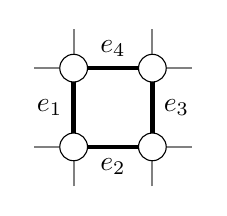
\begin{tikzpicture}
	 		
	 			% Draw axis lines.
				\foreach \y in {1,...,2} {
					\draw[thick, black!50] (0.5, \y) -- (2.5, \y);
				}
				
				\foreach \x in {1,...,2} {
					% Draw vertical axis lines.
					\draw[thick, black!50] (\x, 0.5) -- (\x, 2.5);
				}
				
				% Re-draw edges.
	 			\draw[ultra thick] (1,1) -- (2,1) node[midway,below] {$e_2$};
	 			\draw[ultra thick] (1,1) -- (1,2) node[midway,left] {$e_1$};
	 			\draw[ultra thick] (2,1) -- (2,2) node[midway,right] {$e_3$};
	 			\draw[ultra thick] (1,2) -- (2,2) node[midway,above] {$e_4$};
				
				
				% Draw vertices.
				\foreach \x in {1,...,2} {
	 				\foreach \y in {1,...,2} {
	 					\draw[black, fill=white] (\x, \y) circle (0.5em);
	 				}
	 			}
	 				
	 		\end{tikzpicture}
	 	\end{figure*}
	 	
	 	We want to sample \comment{FIX THIS SHIT!}
	 	
	 	\begin{figure*}[htpb!]
	 		\centering
	 		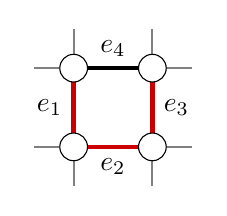
\begin{tikzpicture}
	 		
	 			% Draw axis lines.
				\foreach \y in {1,...,2} {
					\draw[thick, black!50] (0.5, \y) -- (2.5, \y);
				}
				
				\foreach \x in {1,...,2} {
					% Draw vertical axis lines.
					\draw[thick, black!50] (\x, 0.5) -- (\x, 2.5);
				}
				
				% Re-draw edges.
	 			\draw[ultra thick, bured] (1,1) -- (2,1) node[midway,below,black] {$e_2$};
	 			\draw[ultra thick, bured] (1,1) -- (1,2) node[midway,left,black] {$e_1$};
	 			\draw[ultra thick, bured] (2,1) -- (2,2) node[midway,right,black] {$e_3$};
	 			\draw[ultra thick] (1,2) -- (2,2) node[midway,above] {$e_4$};
				
				
				% Draw vertices.
				\foreach \x in {1,...,2} {
	 				\foreach \y in {1,...,2} {
	 					\draw[black, fill=white] (\x, \y) circle (0.5em);
	 				}
	 			}
	 				
	 		\end{tikzpicture}
	 		\caption*{Edges with spin $w_i=1$ are in {\color{bured} red}, while edges with spin $w_i=0$ are in black.}
	 	\end{figure*}
	 	
	 	We can explicitly compute $K((\delta f)(\sigma), 0)$:
	 	\begin{align*}
	 		(\delta f)(\sigma) &= g(\sigma) \\
	 		&= g(e_1 + e_2 + e_3 + e_4) \\
	 		&= g(e_1) + g(e_2) + g(e_3) + g(e_4) \\
	 		&= 1 + 1 + 1 + 0 \\
	 		&= 3 \\
	 		&\equiv 1 \Mod 2,
	 	\end{align*}
	 	
	 	so $\sigma$ is a $1$-plaquette with non-vanishing boundary over $\Z_2$. \question{How many homomorphisms $f$ are there which, given a plaquette $\sigma$, assign it a vanishing boundary? It should be dependent only on the number of edges in $\sigma$, but can we calculate them using something like Stirling numbers? I think we can!}

 	
 	\section*{Probability}
 		We want to conduct experiments on these cell complexes because reasons (magnetism, physics stuff, etc.), so we need a way to sample from them in a precise way.
 		
 		\begin{definitions*}[Random cluster model, Potts lattice gauge theory]
 			Now, let $X$ be a finite $d$-dimensional cell complex (first, we'll address $d=2$ and $d=3$), and let $0 < i < d$. Fix some field $\F$, and choose parameters $p \in [0,1]$ and $q \in (0, \infty)$. The \textit{$i$-plaquette random cluster model on $X$} is the random $i$-complex $P$ containing the full $(i-1)$-skeleton of $X$ according to 
	 		\begin{align*}
	 			\mu_X(P) &= \frac{1}{\mathcal Z} p^{|P|} \cdot (1-p)^{|X^i| - |P|} \cdot q^{\betti(P; \F)_{i-1}} \\
	 			&= p^{(\text{number of plaquettes in } P)} \cdot (1-p)^{(\text{number of plaquettes \textit{not} in }P)} \cdot q^{\betti_{i-1}},
	 		\end{align*}
	 		where $\mathcal Z = \mathcal Z(X,p,q,i,\F)$ is a normalizing constant (to make our distribution ``normal'') and $|X^i|$ and $|P|$ denote the number of $i$-cells of $X$ and $P$, respectively.
	 		
	 		Now, letting $G$ be an arbitrary finite abelian group and $X$ a \textit{cubical complex} (i.e. a sublattice of $\Z^d$ for $1 < d$ an integer), the \textit{$(i-1)$ Potts lattice gauge theory on $X$ with coefficients in $G$} is the measure $$\nu(f) = \frac{1}{\mathcal Z} e^{-\beta \cdot H(f)} = \mu_\beta(f) ,$$ where $\mathcal Z$ is again a normalizing constant and $\beta$ is an inverse temperature parameter. We'll be focusing specifically on the case where $\F \cong \Z_q$, where $q$ is prime (which corresponds to the multiplicative group $\Z(q)$ of $q$\textsuperscript{th} roots of unity in $\C$); when we set $\F = \Z_q$, we call this the \textit{$q$-state Potts lattice gauge theory}. This gives rise to the probability of selecting such a cocycle $f$: $$ \probability{f} = e^{-p \cdot H(f)}. $$
 		\end{definitions*}
 		
 		Special cases of $2$- and $3$-dimensional Potts lattice gauge theory are the Ising model (i.e. $\Z(2)$) and the ``clock'' (i.e. $\Z(3)$) lattice gauge theory.
 		
 		\begin{definition*}[Wilson loop variable]
 			Let $f$ be an $(i-1)$ cocycle. The \textit{generalized Wilson loop variable} associated to the cycle $\gamma \in C_{i-1}(G)$ is the random variable $W_\gamma: C^{i-1}(G; \F_q) \to \C$ is given by $$W_\gamma(f) = (f(\gamma))^\C,$$ where the superscript denotes the ``evaluation'' of $f$ at $\gamma$ in the complex numbers. That is, if $f(\gamma) = g \in \F_q$, $g^\C$ is the corresponding $q$\textsuperscript{th} root of unity in $\C$.
 		\end{definition*}
 		
 		We want to investigate the asymptotics of the Wilson loop variable; to do so, we have a nifty conjecture:
 		
 		\begin{conjecture*}[Area and perimeter laws]
 			Given an inverse temperature $\beta$, a critical inverse temperature $\beta_c$, and a cycle $\gamma$, $$ \expectation{W_\gamma} \propto \begin{cases} e^{-c(\beta) \cdot \perimeter{\gamma}} & \beta > \beta_c \\ e^{-c(\beta) \cdot \area{\gamma}} & \beta < \beta_c \end{cases} $$ where $\perimeter \gamma$ is the number of plaquettes in its support (i.e. the plaquettes in the linear combination) and $\area \gamma$ is the number of plaquettes in the support of its \textit{minimal bounding chain} (i.e. the smallest $(i-1)$-boundary which ``surrounds'' $\gamma$). 
 		\end{conjecture*}
 		
 		An example of the ``perimeter'' and ``area'' concepts are if $i=1$, then $\gamma$ consists of exactly two vertices $\{v,w\}$, its perimeter is $2$, and its area is the distance between $v$ and $w$:
 		
 		\begin{figure*}[htpb!]
 			\centering
 			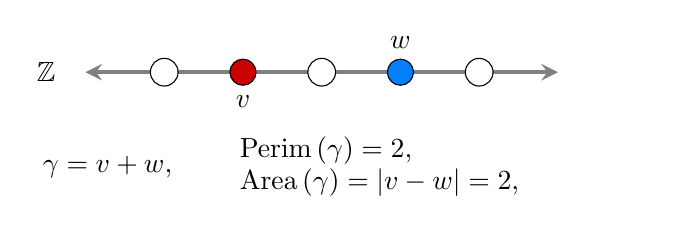
\begin{tikzpicture}
 				\draw node at (-2.5, 0) {$\Z$};
 				\draw[stealth-stealth, black!50, ultra thick] (-2, 0) -- (4, 0);
 				
 				\foreach \x in {-1, 1, 3} {
 					\draw[black, fill=white] (\x, 0) circle (0.5em);
 				}
 				
 				\node[draw, circle, black, fill=bured, minimum size=0.5em, label={below:$v$}] at (0,0) {};
 				\node[draw, circle, black, fill=azure, minimum size=0.5em, label={above:$w$}] at (2,0) {};
 				
 				\node[text width=2in] at (0, -1.2) {$\gamma = v+w$,};
 				\node[text width=2in] at (2.5, -1) {$\perimeter \gamma = 2$,};
 				\node[text width=2in] at (2.5, -1.4) {$\area \gamma = |v-w| = 2$,};
 			\end{tikzpicture}
 		\end{figure*}
 		
 		Now, suppose we have a sublattice $G$ of $\Z^d$ for some $d > 1$, an inverse temperature $\beta$, and a cochain $f \in C^1(G;\Z_q)$. Then, we sample a random $2$-complex $P$ starting with the skeleton (open faces) and including plaquettes $\sigma \in C_2$ such that $(\delta f)(\sigma) = 0$ (i.e. so the spins add up to $0$) with probability $1 - e^{-\beta}$. We get the following theorem (stated above, but more nicely here):
 		
 		\begin{theorem*}[Hiraoka, Shirai]
 			Sampling $P$ from a $q$-state Potts lattice gauge theory gives $$ \probability P \propto p^{(\text{number of plaquettes in } P)} \cdot (1-p)^{(\text{number of plaquettes \textit{not} in }P)} \cdot |H_1(P; \Z_q)|. $$
 		\end{theorem*}
 		
 		Moreover, 
 		
 		\begin{theorem*}
 			Let $\gamma \in C_{i-1}$, and $V_\gamma$ the event that $\partial(\gamma) = 0$ (i.e. $\gamma$ is a cycle) in $H_1(P;\Z_q)$. Then, $$ \expectation{W_\gamma} = \probability{V_\gamma}. $$ Equivalently, the expectation of the Wilson loop variable with respect to $\gamma$ is the same as the probability that $\gamma$ has boundary $0$ over $\Z_q$.
 		\end{theorem*}
 		
 	\section*{Algorithms}
 		The following algorithm, which starts out in $\Z^3$ (i.e. the clock model), tests out these hypotheses: given a cocycle $f \in C^0(G, \Z_2)$, an inverse temperature parameter $-\beta$, and $G$ a sublattice of $\Z_3$, we want to update $f$ in the following way:
 		
 		\begin{enumerate}
 			\item compute $G(f)$, the random graph obtained from evaluating $f$ on $G$, only including plaquettes $\sigma$ such that $(\delta f)(\sigma) = 0$ with probability $p = 1-e^{-\beta}$;
 			\item find the \textit{components} of $G(f)$;
 			\item uniformly randomly assign spins to each of the components of $G(f)$, and call these new spins (i.e. the new cocycle) $f_{\text{new}}$.
 		\end{enumerate}
 		
 		This samples uniformly from $\mu_\beta$. This is called the \textit{Swendson-Wang algorithm}, and is typically used in $\Z^2$ and $\Z^3$; we want to generalize this to higher dimensions.
\end{document}
